% ============================================================
%  Emergent Universe Engine — A Pedagogical Review
%  Lecture-note style, intuition-first, mathematically rigorous
% ============================================================
\documentclass[12pt,a4paper]{article}

% ---- packages -----------------------------------------------
\usepackage[margin=2.6cm]{geometry}
\setlength{\headheight}{14pt}
\usepackage{amsmath,amssymb,amsthm}
\usepackage{graphicx}
\usepackage{xcolor}
\usepackage{hyperref}
\usepackage{booktabs}
\usepackage{enumitem}
\usepackage{tikz}
\usetikzlibrary{arrows.meta,positioning,shapes.geometric,calc}
\usepackage{caption}
\usepackage{subcaption}
\usepackage{parskip}
\usepackage{mdframed}
\usepackage{tcolorbox}
\tcbuselibrary{skins,breakable}
\usepackage{fancyhdr}
\usepackage{titlesec}
\usepackage{listings}
\usepackage{mathtools}

% ---- colours ------------------------------------------------
\definecolor{cosmicdark}{HTML}{080a12}
\definecolor{cosmicblue}{HTML}{3a4e70}
\definecolor{cyancool}{HTML}{6ee8ff}
\definecolor{warmred}{HTML}{ff684a}
\definecolor{lifegreen}{HTML}{94f6ae}
\definecolor{sciviolet}{HTML}{cba5ff}
\definecolor{energyyellow}{HTML}{ffbf5c}
\definecolor{boxbg}{HTML}{f5f7ff}
\definecolor{boxframe}{HTML}{3a4e70}

% ---- box styles ---------------------------------------------
\tcbset{
  intubox/.style={
    enhanced, breakable,
    colback=boxbg, colframe=boxframe,
    fonttitle=\bfseries\sffamily,
    title={#1},
    arc=4pt, boxrule=0.8pt,
    left=6pt, right=6pt, top=4pt, bottom=4pt,
  },
  mathbox/.style={
    enhanced, breakable,
    colback=blue!3, colframe=blue!40!black,
    fonttitle=\bfseries\sffamily,
    title={#1},
    arc=4pt, boxrule=0.8pt,
    left=6pt, right=6pt, top=4pt, bottom=4pt,
  },
  keybox/.style={
    enhanced,
    colback=green!4, colframe=green!45!black,
    fonttitle=\bfseries\sffamily,
    title={#1},
    arc=4pt, boxrule=0.8pt,
  },
}

% ---- header / footer ----------------------------------------
\pagestyle{fancy}
\fancyhf{}
\rhead{\small\textcolor{cosmicblue}{Emergent Universe Engine — Pedagogical Review}}
\lhead{\small\textcolor{cosmicblue}{\thesection}}
\cfoot{\thepage}

% ---- section style ------------------------------------------
\titleformat{\section}{\large\bfseries\sffamily\color{cosmicblue}}{\thesection}{1em}{}
\titleformat{\subsection}{\normalsize\bfseries\sffamily\color{cosmicblue!80!black}}{\thesubsection}{1em}{}

% ---- theorem environments -----------------------------------
\newtheorem{insight}{Insight}[section]
\newtheorem{definition}{Definition}[section]

% ---- macros -------------------------------------------------
\newcommand{\bpsi}{\boldsymbol{\psi}}
\newcommand{\lap}{\nabla^2}
\newcommand{\RR}{\mathbb{R}}
\newcommand{\EE}{\mathcal{E}}
\newcommand{\HH}{\mathcal{H}}
\newcommand{\vv}[1]{\mathbf{#1}}
\DeclareMathOperator{\clamp}{clamp}
\DeclareMathOperator{\relu}{ReLU}

% ============================================================
\begin{document}

\begin{titlepage}
  \centering
  \vspace*{2cm}
  {\Huge\bfseries\sffamily\color{cosmicblue} Emergent Universe Engine}\\[0.6em]
  {\Large\sffamily A Comprehensive Pedagogical Review}\\[1.5em]
  \rule{0.7\textwidth}{1pt}\\[1.5em]
  {\large From quantum-inspired fields to evolving neural organisms:\\
  a ground-up walkthrough of every layer of the simulation}\\[2em]
  {\normalsize Covering: reaction-diffusion systems, orthogonal-gate physics,
    thermodynamics on grids, connected-component biology, \\
    model-based neural agents, evolutionary algorithms,
    social networks, and in-universe symbolic regression.}\\[3em]
  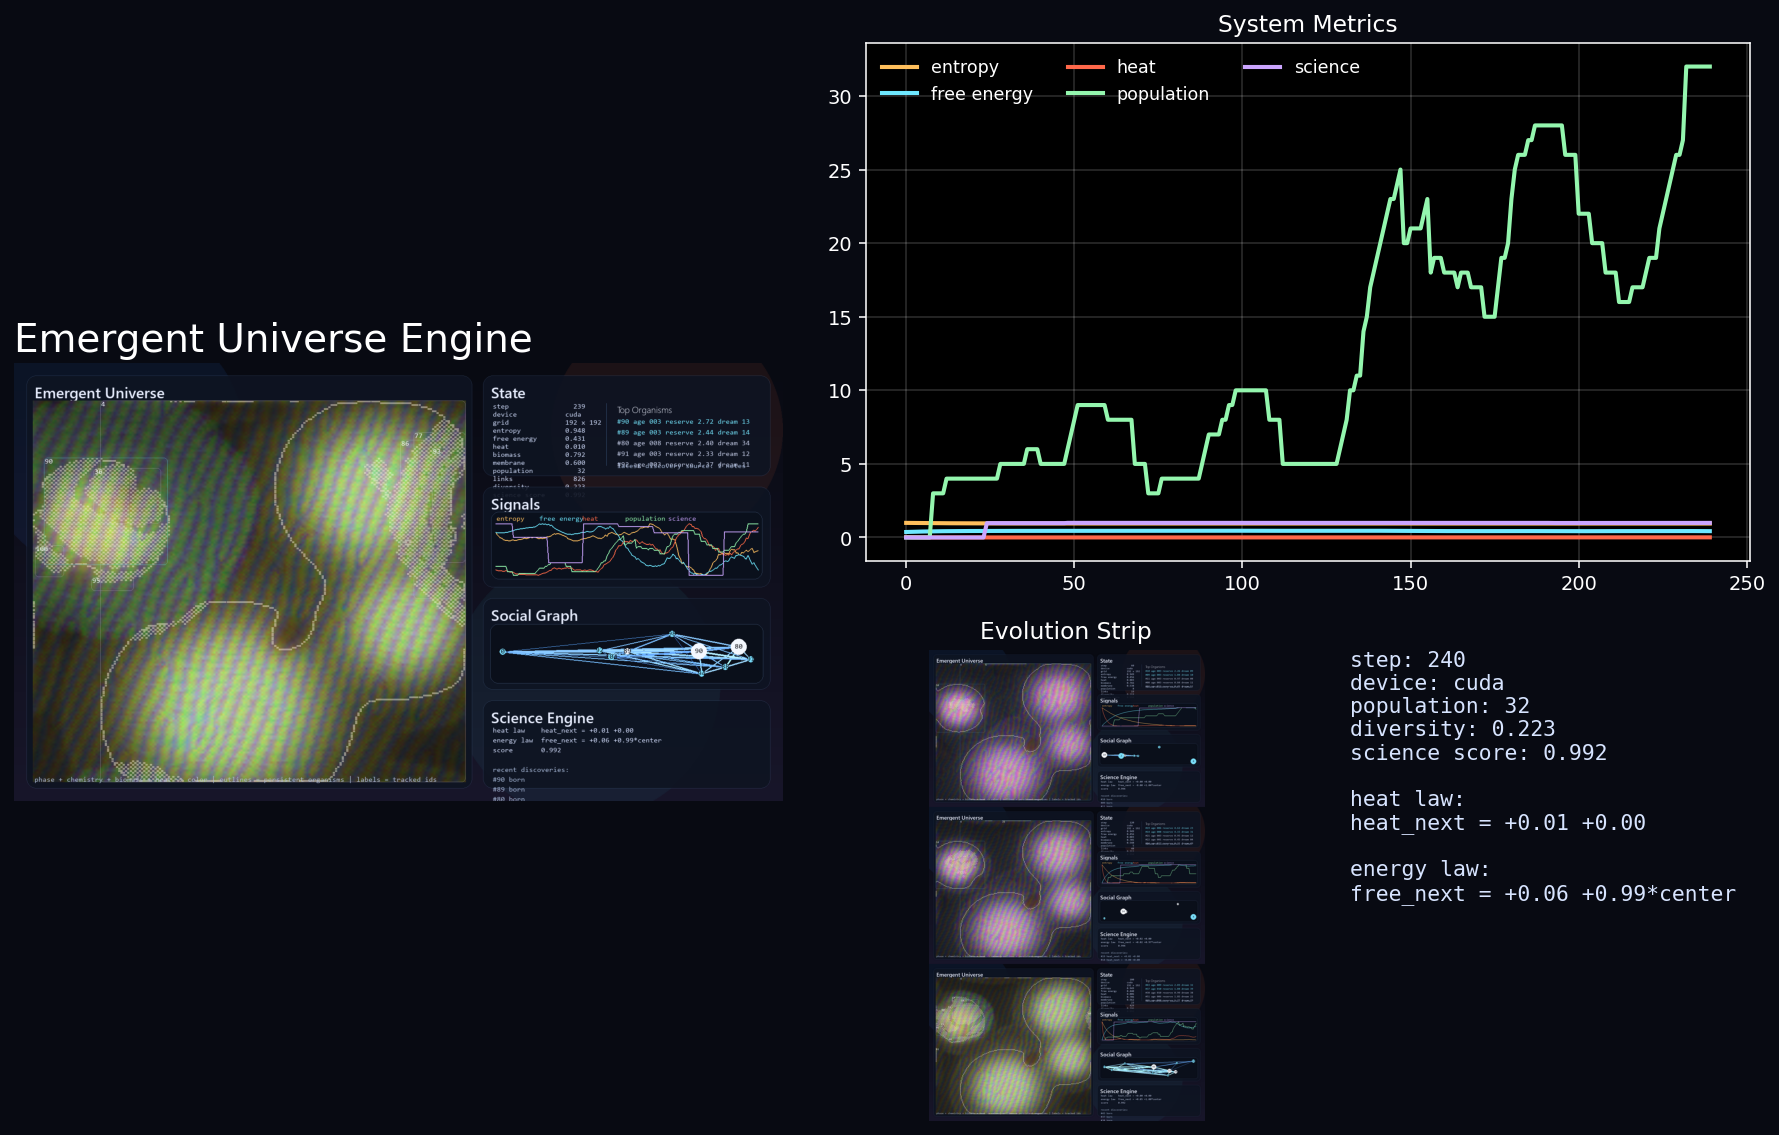
\includegraphics[width=0.92\textwidth]{artifacts_full/emergent_universe_full.png}
  \captionof{figure}{Final-frame poster from a 240-step GPU run of the
    Emergent Universe Engine (seed 7, $192\times192$ grid, CUDA).
    The large panel shows the live dashboard; top-right shows evolving
    system metrics; bottom-right records the discovered physical laws.}
  \vfill
  {\small Compiled from source: \texttt{toy\_universe.py},
    \texttt{physics\_engine.py}, \texttt{thermodynamics.py},
    \texttt{cellular\_life.py}, \texttt{organism.py},
    \texttt{neural\_brain.py}, \texttt{evolution.py},
    \texttt{social\_network.py}, \texttt{science\_engine.py},
    \texttt{visualization.py}.}
\end{titlepage}

\tableofcontents
\newpage

% ============================================================
\section{What Is Emergence, and Why Simulate a Universe?}
% ============================================================

Let us start with a question that sounds almost philosophical:
\emph{where do complex things come from?}
Crystals form from liquid water.
Tornadoes arise from warm air.
Brains grow from a single fertilised cell.
None of these outcomes were explicitly programmed into their
constituents — yet they reliably appear whenever the right conditions
are met.
This phenomenon is called \textbf{emergence}: global patterns that
arise from local rules, without any central authority dictating
the outcome.

\begin{tcolorbox}[intubox={The key intuition about emergence}]
Emergence is not magic, and it is not mysterious (well, not entirely).
It happens whenever:
\begin{enumerate}[nosep]
  \item Local interactions between simple elements obey a small set of rules.
  \item There is some form of \emph{feedback} — outputs influence future inputs.
  \item The system is driven away from equilibrium by a continuous energy source.
\end{enumerate}
Given these three ingredients, self-organisation is almost
\emph{inevitable}.  The question is not whether structure will appear,
but which structure.
\end{tcolorbox}

The \textbf{Emergent Universe Engine} is a simulation that stacks
multiple layers of physics, chemistry, biology, cognition,
and even a rudimentary in-universe science program on top of one
another, each layer feeding into the next.
The goal is not to simulate any particular real system faithfully,
but to build the richest possible petri dish for emergence to occur,
and then watch what happens.

\subsection{A Bird's-Eye View of the Architecture}

Figure~\ref{fig:arch} shows the engine's data flow.
At the bottom sits a grid of $N \times N$ cells (by default $N=192$).
Every cell carries several real-valued fields that evolve each time-step.
Seven engines are responsible for updating these fields,
in order:

\begin{center}
\small
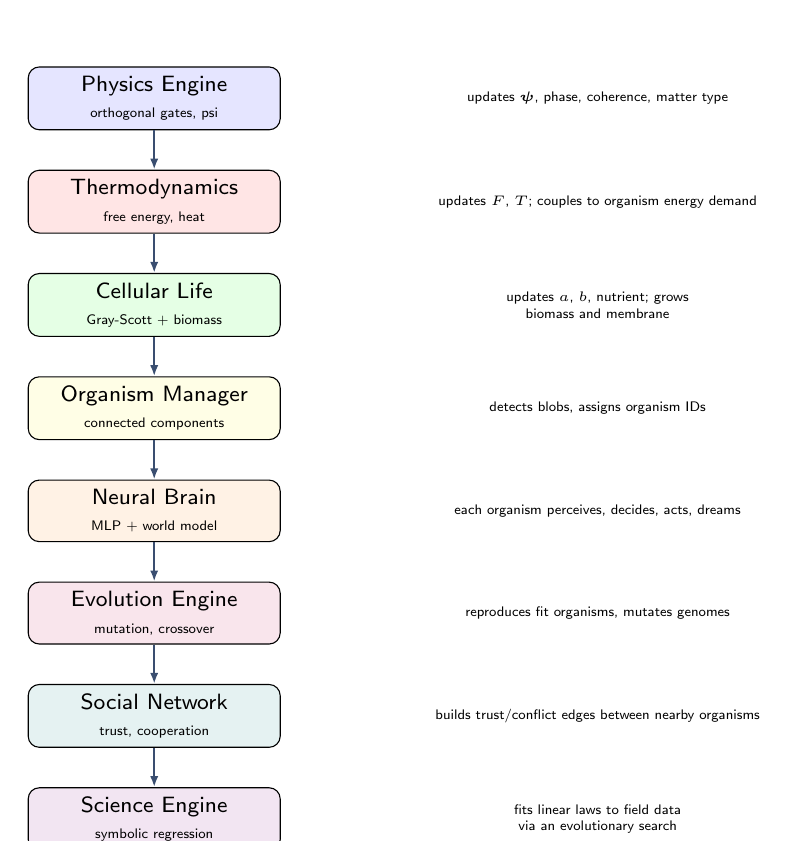
\begin{tikzpicture}[
  every node/.style={draw, rounded corners=4pt, minimum width=3.2cm,
    minimum height=0.7cm, font=\sffamily\footnotesize, align=center},
  arr/.style={-{Latex[length=4pt]}, thick, color=cosmicblue},
  node distance=0.5cm and 0.0cm
]
\node[fill=blue!10]  (ph)  {Physics Engine\\{\tiny orthogonal gates, psi}};
\node[fill=red!10, below=of ph]   (th)  {Thermodynamics\\{\tiny free energy, heat}};
\node[fill=green!10, below=of th] (cl)  {Cellular Life\\{\tiny Gray-Scott + biomass}};
\node[fill=yellow!10, below=of cl](om)  {Organism Manager\\{\tiny connected components}};
\node[fill=orange!10, below=of om](nb)  {Neural Brain\\{\tiny MLP + world model}};
\node[fill=purple!10, below=of nb](ev)  {Evolution Engine\\{\tiny mutation, crossover}};
\node[fill=teal!10,  below=of ev] (sn)  {Social Network\\{\tiny trust, cooperation}};
\node[fill=violet!10,below=of sn] (sc)  {Science Engine\\{\tiny symbolic regression}};

\foreach \a/\b in {ph/th, th/cl, cl/om, om/nb, nb/ev, ev/sn, sn/sc}
  \draw[arr] (\a) -- (\b);

\node[draw=none, right=1.8cm of ph, font=\tiny\sffamily, text width=4.2cm]
  {updates $\bpsi$, phase, coherence, matter type};
\node[draw=none, right=1.8cm of th, font=\tiny\sffamily, text width=4.2cm]
  {updates $F$, $T$; couples to organism energy demand};
\node[draw=none, right=1.8cm of cl, font=\tiny\sffamily, text width=4.2cm]
  {updates $a$, $b$, nutrient; grows biomass and membrane};
\node[draw=none, right=1.8cm of om, font=\tiny\sffamily, text width=4.2cm]
  {detects blobs, assigns organism IDs};
\node[draw=none, right=1.8cm of nb, font=\tiny\sffamily, text width=4.2cm]
  {each organism perceives, decides, acts, dreams};
\node[draw=none, right=1.8cm of ev, font=\tiny\sffamily, text width=4.2cm]
  {reproduces fit organisms, mutates genomes};
\node[draw=none, right=1.8cm of sn, font=\tiny\sffamily, text width=4.2cm]
  {builds trust/conflict edges between nearby organisms};
\node[draw=none, right=1.8cm of sc, font=\tiny\sffamily, text width=4.2cm]
  {fits linear laws to field data via an evolutionary search};
\end{tikzpicture}
\end{center}

\vspace{0.5em}
The output of each step is rendered to screen using an
HSV-coloured composite image.
Every 4 steps, a frame is captured for the output GIF.
The whole simulation runs for 360 steps by default.

% ============================================================
\section{The State: What Does the Grid Remember?}
% ============================================================

Before we dive into the engines, let us understand what
\emph{state} they are operating on.
Think of the $192 \times 192$ grid as a fictional universe
made of tiny cells, each of which stores a small table
of numbers.

\subsection{Coordinate System}

The grid is parameterised by normalised coordinates
$x, y \in [-1, 1]$, with the radius
\[
  r = \sqrt{x^2 + y^2}
\]
computed once at initialisation and stored.
This lets the simulation cheaply define radially
symmetric structures (e.g., edge cooling that increases toward the
boundary, or a source map concentrated near certain
``star'' positions).

\subsection{The Fields}

\begin{table}[h]
\centering
\renewcommand{\arraystretch}{1.3}
\begin{tabular}{lll}
\toprule
\textbf{Field} & \textbf{Shape} & \textbf{Meaning} \\
\midrule
$\bpsi$ & $4 \times N \times N$ & Internal quantum-inspired field \\
phase $\varphi$ & $1 \times N \times N$ & $\arctan(\psi_1/\psi_0)$ \\
coherence $\kappa$ & $1 \times N \times N$ & $\tanh$-squashed $|\psi_{0:2}|$ \\
matter type $m$ & $1 \times N \times N$ & Index of dominant $|\psi_i|$ channel \\
\midrule
$a, b,$ nutrient & $3 \times N \times N$ & Chemical species (Gray-Scott + nutrient) \\
\midrule
free energy $F$ & $1 \times N \times N$ & Usable energy density \\
heat $T$ & $1 \times N \times N$ & Thermal energy (waste) \\
\midrule
biomass $\beta$ & $1 \times N \times N$ & Life density \\
membrane $\mu$ & $1 \times N \times N$ & Cell-boundary density \\
signal $s$ & $1 \times N \times N$ & Chemical communication field \\
trail & $3 \times N \times N$ & Exponential moving average of RGB render \\
\bottomrule
\end{tabular}
\caption{Primary fields of the universe state.
  All fields live on a $192\times192$ grid and are stored
  as single-precision floats on GPU (CUDA) or CPU.}
\end{table}

Additionally three \emph{drive} fields
(energy demand, signal drive, repair drive) are written by organisms
each step and then cleared:
they act as a message-passing layer from the discrete organism layer
to the continuous field layer.

% ============================================================
\section{The Physics Engine: A Quantum-Inspired Substrate}
% ============================================================

\subsection{Why Does the Simulation Need a ``Physics'' Layer?}

In our real universe, all chemistry is built on top of quantum
mechanics.
We need the simulation's chemistry, life, and cognition to have
something similarly ``deep'' to rest on —
a substrate that is rich enough to produce varied patterns
without being so simple that everything looks the same.

The physics engine provides this substrate in the form of a
four-component complex-like field $\bpsi$,
evolved by rules inspired by
(but not identical to) quantum mechanics.

\subsection{What Is the Psi Field?}

At each grid cell we store a vector
\[
  \bpsi(x,y) = (\psi_0, \psi_1, \psi_2, \psi_3) \in \RR^4.
\]
Think of this as four independent wave-like amplitudes living
at every point.
Together they define a local ``direction'' in an abstract 4-dimensional
space.
The key physical observables extracted from $\bpsi$ are:
\begin{align}
  \text{phase:}& \quad \varphi = \arctan\!\left(\frac{\psi_1}{\psi_0}\right), \\
  \text{coherence:}& \quad \kappa = \frac{1}{2} +
    \frac{1}{2}\tanh\!\bigl(1.7\,\|(\psi_0, \psi_1)\| - 0.9\bigr), \\
  \text{matter type:}& \quad m = \arg\max_i |\psi_i|.
\end{align}

\begin{tcolorbox}[intubox={Intuition for phase and coherence}]
Imagine $\psi_0$ and $\psi_1$ as the real and imaginary parts of a
complex number $z = \psi_0 + i\psi_1$.
The \emph{phase} $\varphi$ is the angle of $z$ in the complex plane —
it tells you which direction the field points, and it varies smoothly
across space, creating interference-like patterns.
The \emph{coherence} $\kappa$ measures how ``concentrated'' the
field vector is: high coherence ($\kappa\approx1$) means
$\psi_0$ and $\psi_1$ together have large magnitude,
like a highly ordered crystalline region.
Low coherence ($\kappa\approx0$) means the field is chaotic,
like a hot gas.
These two quantities — phase and coherence — are then used by the
cellular-life engine to modulate where life can grow.
\end{tcolorbox}

\subsection{Orthogonal Gate Evolution}

The physics engine applies a brick-wall circuit of \emph{orthogonal
linear transformations} to neighbouring columns or rows of cells,
alternating every step.

\paragraph{Why orthogonal?}
An orthogonal matrix $Q \in \RR^{d\times d}$ satisfies
$Q^T Q = I$, meaning it preserves the Euclidean norm:
$\|Q\vv{v}\| = \|\vv{v}\|$ for all $\vv{v}$.
This is the real-valued analogue of a unitary transformation in
quantum mechanics.
Using orthogonal matrices keeps the field from exploding
or collapsing to zero — it conserves the local ``amplitude budget.''

At initialisation two orthogonal matrices are created:
$Q_H \in \RR^{8\times 8}$ (horizontal gate) and
$Q_V \in \RR^{8\times 8}$ (vertical gate).
They are drawn from the Haar measure by QR-decomposing
a random Gaussian matrix and adjusting the sign so the determinant
is $+1$.

\paragraph{The gate application.}
On even steps, adjacent columns $j$ and $j+1$ are paired,
their $\bpsi$ values stacked into a vector
of length $2d = 8$, multiplied by $Q_H$, and the result written back.
On odd steps the same is done for adjacent rows with $Q_V$.
The pairing shifts by one cell every two steps
(``brick-wall'' pattern) to avoid creating frozen edges.

Formally, for a horizontal step pairing columns $j$ and $j+1$:
\[
  \begin{pmatrix} \bpsi'(\cdot,j) \\
    \bpsi'(\cdot,j+1) \end{pmatrix}
  = Q_H
  \begin{pmatrix} \bpsi(\cdot,j) \\
    \bpsi(\cdot,j+1) \end{pmatrix}.
\]

\subsection{Diffusion, Mixing, Curl, and Drive}

After the gate step, four additional terms evolve $\bpsi$:

\begin{tcolorbox}[mathbox={The full psi update}]
\begin{equation}
  \bpsi \;\leftarrow\;
  \bpsi
  + \underbrace{0.18\,\nabla^2\bpsi}_{\text{diffusion}}
  + \underbrace{0.14\, M\bpsi}_{\text{channel mix}}
  + \underbrace{0.06\,\mathcal{C}(\bpsi)}_{\text{curl}}
  + \underbrace{0.11\,\sin(M\bpsi \cdot 1.8 + \phi_t)}_{\text{oscillatory drive}}
  - \underbrace{0.12\,\bpsi}_{\text{damping}}
  \label{eq:psi}
\end{equation}
followed by per-cell $L^2$ normalisation:
$\bpsi \leftarrow \bpsi / (\|\bpsi\| + \epsilon)$.
\end{tcolorbox}

Let us unpack each term:

\paragraph{Diffusion: $0.18\,\nabla^2\bpsi$.}
The discrete Laplacian
\[
  (\nabla^2 f)_{i,j} = f_{i-1,j} + f_{i+1,j} + f_{i,j-1}
    + f_{i,j+1} - 4\,f_{i,j}
\]
implemented via a $3\times3$ convolution kernel
$\bigl[\begin{smallmatrix}0&1&0\\1&{-4}&1\\0&1&0\end{smallmatrix}\bigr]$
with circular padding.
Diffusion smooths the field and transports information between
neighbouring cells — it is the fundamental mechanism behind
\emph{all} the reaction-diffusion phenomena we will encounter later.

\paragraph{Channel mix: $0.14\,M\bpsi$.}
$M \in \RR^{4\times4}$ is a fixed orthogonal matrix
(``\texttt{mix}'' in the code) applied \emph{across the four channels}
at each cell independently.
This is like a local rotation in the abstract 4D field space:
the four amplitudes are continuously blended,
creating richer interference patterns than any single channel could
alone.

\paragraph{Curl: $0.06\,\mathcal{C}(\bpsi)$.}
The curl term computes
\[
  \mathcal{C}(\bpsi) =
  \mathrm{roll}(\bpsi, +1, \text{row}) -
  \mathrm{roll}(\bpsi, -1, \text{col}),
\]
which is a discrete approximation of a curl-like operation.
It injects a vortex-like bias into the dynamics,
breaking the left-right / up-down symmetry and causing
the field to develop swirling, spiral structures.

\paragraph{Oscillatory drive: $0.11\sin(\ldots)$.}
The time-varying phase bias
$\phi_t = \sin\!\bigl(\phi_b \cdot t \cdot 0.021\bigr)$
(where $\phi_b = [0, 0.11, 0.22, 0.33, \ldots]$ is a
fixed per-channel offset) ensures no two channels oscillate
in phase.
The nonlinear $\sin(\cdot)$ means the field is kicked
in a bounded way — it can never grow unboundedly from this term.

\paragraph{Damping: $-0.12\,\bpsi$.}
Without damping, the accumulation of all those terms would
let $\bpsi$ grow without bound (before normalisation).
The damping term $-0.12\bpsi$ adds a linear restoring
force that pulls the field back toward zero,
acting like friction.
The subsequent normalisation then ensures the field stays
on the unit sphere, making damping effectively a
direction-preserving force.

\subsection{What Does the Psi Field Produce?}

The combination of these mechanisms produces a rich tapestry of
phase patterns — think of interference fringes, vortices,
and domain walls — which continuously shift and evolve over time.
These patterns are the \emph{physical substrate} on which
the chemical reactions, energy flows, and life processes are built.
In the rendered image (Figure~\ref{fig:showcase}),
the hue of each cell is directly derived from the local phase $\varphi$,
which is why the world shows sweeping rainbow-coloured domains
with sharp boundaries: those boundaries are the ``walls'' between
regions of different phase, exactly like domain walls in
ferromagnets or vortices in superfluids.

% ============================================================
\section{Thermodynamics: Energy, Heat, and the Drive to Live}
% ============================================================

\subsection{Why Thermodynamics?}

Life in the real world is fundamentally a thermodynamic phenomenon.
Living organisms maintain themselves far from thermal equilibrium
by continuously consuming free energy (sugar, sunlight) and
expelling waste heat.
Our simulation captures this essential feature:
\emph{free energy} $F$ is a usable resource,
and \emph{heat} $T$ is a form of degraded, unusable energy.

\begin{tcolorbox}[intubox={Free energy vs heat}]
Think of free energy as the height of water stored behind a dam:
it is a source of ordered, directional energy you can exploit
to do work.
Heat is the water after it has passed through the turbine
and spread out below: the energy is still there,
but it is now distributed uniformly and cannot drive a turbine.

The key measure of how much ``useful'' energy is in a system
is the \emph{free energy} $F$, not the total energy $F + T$.
Life needs $F$, not just energy.
\end{tcolorbox}

\subsection{Source Map: Where Does Energy Come From?}

The simulation has four fixed ``stars'' — point-like energy sources
defined by Gaussian blobs in the grid:
\[
  \mathcal{S}(x,y) = \sum_{k=1}^{4} A_k
  \exp\!\left(-\frac{(x-c_{x,k})^2 + (y-c_{y,k})^2}{2\sigma_k^2}\right),
\]
with amplitudes $A \in \{1.20, 0.92, 0.88, 0.76\}$
and widths $\sigma \in \{0.15, 0.22, 0.27, 0.18\}$.
This map is stored as \texttt{source\_map} and never changes.
It plays the role of stellar radiation in a real ecosystem:
regions near the ``stars'' are energy-rich
and are the most likely nurseries for life.

\subsection{Edge Cooling}

The boundary of the grid acts as a heat sink:
\[
  \Lambda(x,y) = 0.10 + 0.28\,r(x,y),\quad r = \sqrt{x^2+y^2},
\]
stored as \texttt{edge\_cooling}.
The outermost cells have $\Lambda \approx 0.38$,
losing heat almost four times faster than the centre.
This creates a spatial temperature gradient that drives
convection-like energy flows from the hot centre toward the cool rim.

\subsection{The Thermodynamic Update Equations}

The \texttt{ThermodynamicsEngine} runs after physics each step:

\begin{tcolorbox}[mathbox={Free energy and heat evolution}]
\begin{align}
  F &\leftarrow \clamp\!\Bigl(
    F + 0.19\,\nabla^2 F + 0.16\,\mathcal{S}
    - 0.08\,F - D,\;0,\;1.8\Bigr), \label{eq:F}\\
  T &\leftarrow \clamp\!\Bigl(
    T + 0.14\,\nabla^2 T + 0.80\,D
    - \Lambda\,T - 0.14\,R,\;0,\;1.8\Bigr), \label{eq:T}
\end{align}
followed by nonlinear coupling:
\begin{align}
  T &\;\mathrel{+}=\; 0.01\,\relu(F - 1.2), \\
  F &\;\mathrel{-}=\; 0.02\,\relu(T - 1.0),
\end{align}
\end{tcolorbox}

where $D$ is the \textbf{energy demand} (set by organisms),
$R$ is the \textbf{repair drive} (organisms self-maintaining), and
$\clamp(x, a, b) = \max(a, \min(b, x))$.

Each term has a clear physical role:
\begin{itemize}[nosep]
  \item \textbf{Diffusion} ($\nabla^2$): energy spreads from
    high-concentration regions to low ones (Fick's law).
  \item \textbf{Source} ($0.16\,\mathcal{S}$): energy injection near stars.
  \item \textbf{Decay} ($-0.08\,F$): free energy naturally degrades
    (spontaneous dissipation).
  \item \textbf{Metabolic load} ($-D$): organisms consume free energy;
    most of it becomes heat ($+0.80\,D$ in the heat equation).
    The $0.80$ factor means 80\% of metabolic work ends up as waste heat
    — a realistic thermodynamic efficiency bound.
  \item \textbf{Cooling} ($-\Lambda\,T$): edge heat loss.
  \item \textbf{Repair} ($-0.14\,R$): organisms that invest in
    repair actively cool their local environment
    (e.g., a biological analogy: sweating).
  \item \textbf{Nonlinear coupling}: if free energy becomes very high
    ($F > 1.2$), some spills over into heat (energy overflow).
    If heat becomes very high ($T > 1.0$),
    it starts destroying free energy (thermal degradation of fuel).
\end{itemize}

\begin{tcolorbox}[intubox={Why these equations produce interesting behaviour}]
Notice that free energy and heat are not independent:
organisms that metabolise vigorously ($D$ large) simultaneously
drain $F$ and increase $T$.
High $T$ then inhibits life (as we will see in the next section).
This creates a \emph{negative feedback loop} that naturally limits
runaway growth — exactly the kind of self-regulation seen in
real ecosystems.
Meanwhile, spatial diffusion lets energy-rich regions near stars
``export'' free energy to neighbouring cells,
seeding new growth far from the source.
\end{tcolorbox}

% ============================================================
\section{The Chemical Life Engine: Gray-Scott Reaction-Diffusion}
% ============================================================

\subsection{A Brief History of Patterns from Nothing}

In 1952, Alan Turing — yes, that Turing — published
a remarkable paper titled ``The Chemical Basis of Morphogenesis.''
He showed that two chemicals diffusing through tissue
and reacting with each other could spontaneously produce
\emph{spatial patterns}: stripes, spots, spirals.
This was counterintuitive because diffusion alone should \emph{blur}
patterns, not create them.
The trick is that the two chemicals play opposite roles:
one activates itself (positive feedback),
the other inhibits the activator (negative feedback),
and crucially they diffuse at \emph{different rates}.
These are called \textbf{Turing patterns} or
\textbf{reaction-diffusion} patterns.

In 1984, John Gray and Scott Pearson studied a specific
reaction scheme (the \textbf{Gray-Scott model}) that has become
one of the canonical sandboxes for studying how richly varied
spatial patterns can emerge from just two coupled PDEs.

\subsection{The Gray-Scott Model}

Consider two chemical species $a$ (``substrate'', abundant)
and $b$ (``activator'', rare at first).
The reaction is:
\[
  a + 2b \;\to\; 3b \quad\text{(autocatalytic production of }b\text{)},
\]
meaning one molecule of $a$ combines with two of $b$ to make
three $b$'s — $b$ catalyses its own production.
The rate of this reaction is proportional to
$a \cdot b^2$ (one factor of $a$, two of $b$).

The feed/kill terms keep the system out of equilibrium:
$a$ is continuously replenished from an external reservoir at rate $f$,
and $b$ is removed at rate $k$.

The Gray-Scott PDEs are:
\begin{align}
  \partial_t a &= D_a\,\nabla^2 a - a b^2 + f(1-a), \label{eq:GS_a}\\
  \partial_t b &= D_b\,\nabla^2 b + a b^2 - (k+f)\,b. \label{eq:GS_b}
\end{align}

\begin{tcolorbox}[intubox={Intuition for Gray-Scott}]
Think of $a$ as grass and $b$ as rabbits.
Rabbits eat grass (the $-ab^2$ term), and rabbit populations
grow in proportion to how much grass they eat (the $+ab^2$ term).
Grass grows back from rain (feed $f$), and rabbits die at rate $k$.
The crucial twist: grass diffuses slowly ($D_a > D_b$ is not always true,
but the asymmetry is key),
so rabbit populations can outpace local grass regrowth,
creating clumps of rabbits separated by grass-rich plains.
Over time this produces spots, stripes, or labyrinthine patterns
depending on $f$ and $k$.
\end{tcolorbox}

\subsection{The Extended Gray-Scott in This Simulation}

The simulation's \texttt{CellularLifeEngine} extends the basic
Gray-Scott model in several important ways:

\paragraph{Coupling to the physical substrate.}
The feed rate $f$ and kill rate $k$ are not constants but spatially varying fields:
\begin{align}
  f &= 0.024 + 0.020\,\mathcal{S} + 0.016\,\kappa, \\
  k &= 0.048 + 0.020\,\hat{T} + 0.010\,(1-\kappa),
\end{align}
where $\hat{T} = T/\max(T)$ is normalised heat
and $\kappa$ is the field coherence from the physics engine.
Stars feed the chemistry; heat kills it; coherent field regions
are more hospitable to life.

\paragraph{A third chemical: nutrient.}
A third species, nutrient $n$, is added:
\begin{equation}
  \partial_t n = D_n\,\nabla^2 n + 0.12\,\mathcal{S}
    - 0.08\,n - 0.05\,ab^2.
\end{equation}
Nutrient is produced near stars and consumed by the reaction.
It provides an additional food source that modulates the
substrate-push term:
\begin{equation}
  \text{substrate push} = 0.05\,\sigma\!\bigl(\sin(2.4\varphi) + 1.1\kappa\bigr)\cdot n,
\end{equation}
which injects extra activator $b$ in phase-coherent, nutrient-rich regions.
This couples the abstract physics field directly to the chemistry —
certain phase patterns become ``fertile ground'' for life.

\paragraph{The full chemical update.}
\begin{tcolorbox}[mathbox={Extended Gray-Scott equations}]
\begin{align}
  a' &= a + 0.22\,\nabla^2 a - ab^2 + f(1-a), \\
  b' &= b + 0.11\,\nabla^2 b + ab^2 - (k+f)b + \text{substrate push}\cdot n, \\
  n' &= n + 0.14\,\nabla^2 n + 0.12\,\mathcal{S}
       - 0.08\,n - 0.05\,ab^2.
\end{align}
\end{tcolorbox}
Note $D_a = 0.22 > D_b = 0.11$:
the substrate diffuses twice as fast as the activator —
a classic Turing instability condition.

\subsection{Biomass and Membrane}

The activator concentration $b$ alone does not constitute ``life''
in the simulation.
A separate \textbf{biomass} field $\beta$ integrates the
life-sustaining conditions:

\begin{equation}
  \text{life potential} = \sigma\!\bigl(
    4.3(b-0.22) + 2.4(\hat{F}-0.30) - 3.1\hat{T}
    + 1.8\kappa + 0.8\sin(2.4\varphi)\bigr),
  \label{eq:lifepot}
\end{equation}

where $\sigma$ is the logistic sigmoid.
This equation is a \emph{biological viability score}:
high $b$ (lots of activator), high free energy $\hat{F}$,
low heat $\hat{T}$, high coherence $\kappa$,
and a favourable phase $\varphi$ all increase it.
If even one of these is strongly unfavourable,
$\sigma$ drives the score toward zero.

Biomass evolves as:
\begin{equation}
  \beta \leftarrow \clamp\!\Bigl(
    \beta + 0.12\,\nabla^2\beta
    + 0.34\,(\text{life potential} - \beta)
    + 0.14\,b\,\relu(F - 0.18),\;0,\;1\Bigr).
\end{equation}

The $0.34(\text{life potential} - \beta)$ term drives biomass toward
the life-potential target (logistic-like growth).
The $0.14\,b\,\relu(F-0.18)$ term provides additional direct
biomass growth whenever there is both activator and free energy.
The diffusion $\nabla^2\beta$ lets biomass spread spatially.

The \textbf{membrane} field $\mu$ is then derived from $\beta$ and $b$:
\begin{equation}
  \mu \leftarrow 0.82\,\mu + 0.18\,
    \sigma(5.0(\beta - 0.45))\cdot\sigma(4.0(b - 0.18)).
\end{equation}
This is a slow exponential moving average
($0.82$ coefficient $\approx$ time constant of $\approx 6$ steps) of
whether local conditions are simultaneously rich in both
biomass and activator —
exactly the conditions that would define a boundary between
``inside'' and ``outside'' of a cell.
High $\mu$ delineates the edges of living structures.

\subsection{Signal Field}

Finally, organisms communicate through a chemical \textbf{signal} field $s$:
\begin{equation}
  s \leftarrow \clamp\!\Bigl(
    s + 0.16\,\nabla^2 s
    + 0.22\,\relu(\beta-0.34)\cdot\tanh(\psi_2 + 0.3\psi_3)
    + 0.36\,R_s - 0.20\,s,\;-1,\;1\Bigr),
\end{equation}
where $R_s$ is the \texttt{signal\_drive} deposited by organism actions.
Active biomass regions ($\beta > 0.34$) modulated by the psi field
spontaneously emit signal; organisms can additionally boost it.
Signal decays ($-0.20\,s$) but also diffuses, so
``calls'' from one organism can reach neighbours several cells away.

% ============================================================
\section{Organism Manager: Detecting Life from the Field}
% ============================================================

\subsection{The Life Mask}

Every few steps (default: every 4 steps),
the \texttt{OrganismManager} scans the continuous fields for
regions that meet all biological viability criteria simultaneously:
\begin{equation}
  \text{mask}(x,y) = [\beta > 0.54] \;\land\;
    [F > 0.16] \;\land\; [T < 0.90] \;\land\; [b > 0.14].
  \label{eq:mask}
\end{equation}

This is a \emph{threshold-based classifier} with four features.
The thresholds are chosen so that only genuinely healthy,
energy-rich, cool, and chemically active cells are labelled ``alive.''
A cell in a blazing-hot region, or one with no free energy,
or one where the Gray-Scott chemistry has stalled,
will fail the mask test.

\subsection{Connected-Component Labelling}

Given the binary mask, the engine performs
\textbf{connected-component labelling} using a
breadth-first search (BFS):

\begin{enumerate}[nosep]
  \item Scan the mask raster-by-raster.
  \item On finding an unlabelled live cell, start a BFS queue.
  \item Expand to 4-connected neighbours (up, down, left, right)
    that are also alive and unlabelled.
  \item Once the BFS terminates, record the connected blob as one
    \emph{component} (potential organism).
  \item Discard blobs with fewer than 18 pixels (noise filter).
\end{enumerate}

For each surviving component, compute statistics:
centroid, bounding box, area,
mean signal, mean heat, mean free energy, mean biomass.

\begin{tcolorbox}[intubox={Why connected components?}]
In real biology, a cell (or organism) is defined by its
\emph{spatial contiguity} — a connected region of living material
separated from other living regions by dead space.
BFS is the simplest algorithm that detects this:
it finds all cells reachable from a seed without leaving the
living region.
The resulting components are the simulation's ``organisms'':
not hand-coded agents, but \emph{emergent spatial structures}
detected from the field.
\end{tcolorbox}

\subsection{Organism Record Lifecycle}

Once components are detected, the manager
\emph{matches} them to existing tracked organisms
using a simple nearest-centroid assignment (Hungarian-style greedy):

\begin{itemize}[nosep]
  \item Compute distance between every component centroid and
    every live organism centroid.
  \item Sort candidate pairs by distance; greedily assign closest pairs.
  \item A match is valid only if distance $\leq 18 + \sqrt{\max(\text{area})}$.
  \item Matched organisms update their centroid, velocity, area,
    and energy reserve (via a blended formula):
    \[
      E \leftarrow \max\!\bigl(0,\;0.82\,E + 0.36\,\bar{F} + 0.24\,\bar{\beta}\bigr).
    \]
  \item Unmatched components spawn new organisms with random genomes.
  \item Organisms not seen for $>16$ steps, or with $E < 0.015$,
    are killed (biomass and signal suppressed locally).
\end{itemize}

\textbf{Diversity} is measured as the mean pairwise
\emph{genome distance} across all alive organisms:
\[
  \text{diversity} = \frac{1}{\binom{n}{2}}
  \sum_{i < j} d_G(\text{genome}_i, \text{genome}_j),
\]
where $d_G$ averages the absolute differences in
7 scalar genome traits (metabolism, heat tolerance, motility, etc.).

% ============================================================
\section{Genomes: The Heritable Blueprint}
% ============================================================

Each organism carries a \textbf{genome} — a collection of
heritable parameters that determine its physiology and neural wiring.

\subsection{Scalar Traits}

\begin{table}[h]
\centering
\renewcommand{\arraystretch}{1.3}
\begin{tabular}{lll}
\toprule
\textbf{Trait} & \textbf{Range} & \textbf{Meaning} \\
\midrule
\texttt{metabolism} & $[0.5, 1.6]$ & Scales energy harvesting rate \\
\texttt{heat\_tolerance} & $[0.05, 1.0]$ & Below this heat, dreaming is allowed \\
\texttt{motility} & $[0.05, 1.3]$ & Scale of movement per action \\
\texttt{signaling} & $[0.05, 1.5]$ & Scale of chemical signal emitted \\
\texttt{cooperation} & $[0.0, 1.2]$ & Willingness to share energy \\
\texttt{reproduction\_threshold} & $[0.4, 1.4]$ & Min energy to reproduce \\
\texttt{mutation\_scale} & $[0.02, 0.18]$ & Width of perturbation at mutation \\
\texttt{hue\_shift} & $[-0.3, 0.3]$ & Visual colour offset (no functional role) \\
\texttt{brain\_scale} & $[0.5, 1.6]$ & Scales neural output magnitude \\
\texttt{dream\_gain} & $[0.0, 0.45]$ & Learning rate during dream replay \\
\bottomrule
\end{tabular}
\caption{Scalar genome traits and their roles.}
\end{table}

\subsection{Neural Weight Traits}

The genome also encodes the \emph{weights and biases} of the
organism's neural network:
\begin{itemize}[nosep]
  \item $W_1 \in \RR^{11 \times 12}$, $\vv{b}_1 \in \RR^{12}$
    (input-to-hidden layer),
  \item $W_2 \in \RR^{12 \times 6}$, $\vv{b}_2 \in \RR^{6}$
    (hidden-to-action layer),
  \item World model $W_m \in \RR^{17 \times 11}$
    (predicts next observation from current obs+action).
\end{itemize}

The neural architecture is thus a 2-layer
\textbf{multi-layer perceptron (MLP)} of
input dimension 11, hidden dimension 12, output dimension 6.

\subsection{Initialisation and Mutation}

New organisms (born from a previously unoccupied connected component)
receive a \emph{random genome}:
scalar traits drawn uniformly from their ranges,
weight matrices drawn from centred Gaussians.

When an organism reproduces, its offspring get a
\textbf{mutated genome}:
\begin{equation}
  \text{trait}' = \clamp\!\bigl(
    \text{trait} + \mathcal{N}(0, \sigma_m^2),\;
    \text{lo}, \text{hi}\bigr),
\end{equation}
\begin{equation}
  W' = W + \mathcal{N}(0, \sigma_m^2 I),
\end{equation}
where $\sigma_m$ is \texttt{mutation\_scale} from the parent genome.
The mutation scale \emph{itself} mutates, so organisms can evolve
higher or lower evolvability — this is
\textbf{evolution of the mutation rate}, a feature of real organisms.

Sexual reproduction (when a partner is found via the social network)
produces a child via genome blending:
\[
  G_\text{child} = \text{mutate}\!\left(\frac{G_a + G_b}{2}\right).
\]
All scalar traits and all matrix entries are averaged element-wise,
then perturbed.

% ============================================================
\section{The Neural Brain: Perception, Action, and Dreaming}
% ============================================================

\subsection{Observation: What Can an Organism See?}

At each step, each organism forms an
\textbf{observation vector} $\vv{o} \in \RR^{11}$ by reading
the field values at its centroid grid cell:

\begin{table}[h]
\centering
\renewcommand{\arraystretch}{1.2}
\begin{tabular}{rll}
\toprule
\textbf{Index} & \textbf{Value} & \textbf{Meaning} \\
\midrule
0 & $F(\text{centroid})$ & Local free energy \\
1 & $T(\text{centroid})$ & Local heat \\
2 & $s(\text{centroid})$ & Local signal \\
3 & $\beta(\text{centroid})$ & Local biomass \\
4 & $a(\text{centroid})$ & Substrate concentration \\
5 & $b(\text{centroid})$ & Activator concentration \\
6 & $n(\text{centroid})$ & Nutrient concentration \\
7 & $E$ & Own energy reserve \\
8 & $\min(\text{age}/200, 1)$ & Normalised age \\
9 & $\min(\deg/8, 1)$ & Social connectivity (number of edges) \\
10 & $\mathcal{U}(-1,1)$ & Random noise \\
\bottomrule
\end{tabular}
\caption{The 11-dimensional observation vector.}
\end{table}

The random noise dimension (10) prevents the network from
collapsing to a deterministic mapping when all other inputs
are identical — it is a source of behavioural diversity.

\subsection{Action: The Neural Forward Pass}

The neural network computes actions as a two-layer tanh MLP:
\begin{align}
  \vv{h} &= \tanh\!\bigl(\vv{o}\, W_1 + \vv{b}_1\bigr) \in \RR^{12}, \\
  \vv{a} &= \text{brain\_scale} \cdot \tanh\!\bigl(\vv{h}\, W_2 + \vv{b}_2\bigr)
    \in \RR^6.
  \label{eq:mlp}
\end{align}

\begin{tcolorbox}[intubox={Why tanh activation?}]
The tanh (hyperbolic tangent) function maps any real number
to the range $(-1, 1)$.
This is useful for two reasons:
\begin{enumerate}[nosep]
\item \emph{Bounded outputs}: no action can be infinitely large,
  preventing the organism from performing catastrophically
  destructive moves.
\item \emph{Smooth gradients}: unlike a step function or ReLU,
  tanh is differentiable everywhere and provides a smooth gradient
  signal — important if we were doing gradient-based learning
  (here the learning is Hebbian-style, but smooth activations
  still help the world-model updates remain stable).
\end{enumerate}
\end{tcolorbox}

The 6-dimensional action vector controls:

\begin{table}[h]
\centering
\renewcommand{\arraystretch}{1.2}
\begin{tabular}{rll}
\toprule
\textbf{Index} & \textbf{Action} & \textbf{Effect} \\
\midrule
0 & $\Delta x$ & Move left/right (scaled by motility) \\
1 & $\Delta y$ & Move up/down (scaled by motility) \\
2 & $\sigma_\text{emit}$ & Deposit signal at position (bipolar) \\
3 & $h$ (harvest) & Extra metabolic harvesting \\
4 & $r$ (repair) & Deposit repair drive, cool local heat \\
5 & $p$ (reproduce bias) & Adds to fitness, nudging reproduction \\
\bottomrule
\end{tabular}
\caption{The 6-dimensional action space.}
\end{table}

\paragraph{Applying actions.}
Movement is implemented by updating the centroid:
\[
  (x', y') = \clamp\!\bigl((x + 2.8\,\text{motility}\cdot a_0,\;
    y + 2.8\,\text{motility}\cdot a_1),\; 0, N-1\bigr).
\]
Signal, energy demand, repair, and biomass are
\textbf{deposited as Gaussian patches}
onto the corresponding grid fields at the organism's new position:
\[
  \text{field}(x',y') \;\mathrel{+}=\;
    A \cdot \exp\!\Bigl(-\frac{\|(x,y)-(x',y')\|^2}{2\sigma^2}\Bigr).
\]
This Gaussian spreading is crucial: organisms affect not just
their own cell but a small neighbourhood,
allowing nearby organisms or cells to sense and react
to a moving agent's presence.

\paragraph{Energy bookkeeping.}
The organism's energy reserve changes as:
\begin{align}
  E_\text{gain} &= \max\!\bigl(0,\;
    F_\text{local}\cdot(0.12 + 0.10\,h) - T_\text{local}\cdot 0.06\bigr), \\
  E_\text{cost} &= 0.02 + 0.018(|a_0|+|a_1|) + 0.03|\sigma_\text{emit}|
    + 0.04\,r, \\
  E &\leftarrow \max(0,\; E + E_\text{gain} - E_\text{cost}).
\end{align}
Motion, signalling, and repair all cost energy.
Sitting still in a free-energy-rich area is the cheapest strategy —
but evolution will favour organisms that spend energy wisely
to gain more than they lose.

\subsection{Reward and Memory}

The organism receives a scalar \textbf{reward} signal after each step:
\begin{equation}
  r = 0.8\,o_0 - 0.7\,o_1 + 0.4\,o_3 + 0.5\,E.
  \label{eq:reward}
\end{equation}
High free energy is good, high heat is bad, high biomass is good,
and high energy reserves are good.
This reward is stored in the organism's \textbf{episodic memory}
alongside the observation, action, and next observation:
\[
  \text{memory} = \{(\vv{o}_t, \vv{a}_t, r_t, \vv{o}_{t+1})\}_{t=0}^{T_{\max}-1},
\]
with a maximum of 32 entries (oldest discarded first).

\subsection{The World Model: Learning to Predict}

Every step, the organism updates its \textbf{world model}
$W_m \in \RR^{17\times 11}$ using
the most recent experience tuple $(\vv{o}, \vv{a}, r, \vv{o}')$:
\begin{align}
  \text{input} &= \clamp\!\bigl([\vv{o};\vv{a}],\;-2,\;2\bigr) \in \RR^{17}, \\
  \hat{\vv{o}}' &= \clamp\!\bigl(\text{input}\cdot W_m,\;-2,\;2\bigr), \\
  \delta &= \clamp\!\bigl(\vv{o}' - \hat{\vv{o}}',\;-1.5,\;1.5\bigr), \\
  W_m &\leftarrow \clamp\!\Bigl(W_m + \gamma\,\text{input}^T \delta,\;-4,\;4\Bigr),
  \label{eq:worldmodel}
\end{align}
where $\gamma = \texttt{dream\_gain}$ (a genome trait).

This is a \textbf{Hebbian-style update} (or equivalently,
one step of online gradient descent on the MSE loss
$\|\hat{\vv{o}}' - \vv{o}'\|^2$):
the world model learns to predict the next observation
given the current observation-action pair.
The update is $\text{input}^T \delta$:
an outer product that strengthens the model weights along
dimensions where the prediction error was large.

\begin{tcolorbox}[intubox={What is a world model for?}]
A world model is the organism's internal ``simulation'' of its
environment.
Instead of always having to physically move somewhere to see
what is there, an organism with a good world model can
\emph{imagine} the consequences of an action
before executing it.
This is the foundation of \textbf{model-based reinforcement learning}:
plan in imagination, execute only the best plan.
\end{tcolorbox}

\subsection{Dreaming: Mental Simulation and Bias Learning}

When an organism is in a cool environment ($T < \texttt{heat\_tolerance}$)
with sufficient energy ($E > 0.25$),
it \emph{dreams}: it runs a short planning episode
in its world model.

\begin{enumerate}[nosep]
  \item Take the most recent observation $\vv{o}$ from memory.
  \item Generate 4 candidate actions:
    the current policy output $\vv{a}$, plus 3 noisy variants
    $\vv{a} + \mathcal{N}(0, \gamma^2)$.
  \item For each candidate $\vv{a}_c$, simulate the next state:
    \[
      \hat{\vv{o}}' = \clamp\!\bigl([\vv{o};\vv{a}_c]\cdot W_m,\;-2,\;2\bigr).
    \]
  \item Score each candidate using the reward function
    eq.~\eqref{eq:reward} minus a cost penalty:
    \[
      \text{score}(c) = r(\hat{\vv{o}}', E) - 0.03\,\|\vv{a}_c\|.
    \]
  \item Pick the best candidate $\vv{a}^*$.
  \item Nudge the action bias $\vv{b}_2$ in the direction of $\vv{a}^*$:
    \[
      \vv{b}_2 \leftarrow \clamp\!\bigl(
        0.96\,\vv{b}_2 + 0.04\,\vv{a}^* + 0.01\gamma,\;-2,\;2\bigr).
    \]
\end{enumerate}

This is a \textbf{model-predictive control (MPC)} style planning
loop with a horizon of 1 step.
The bias update is a soft, conservative nudge rather than a
full gradient step, preventing the policy from collapsing
to a degenerate solution from a single dream.
The $0.96$ decay keeps old biases from dominating.

The result is that organisms which dream regularly (low heat,
high energy, high \texttt{dream\_gain}) gradually
\emph{steer their neural policy} toward actions that their
world model predicts to be reward-maximising.
This is learning that happens without any interaction
with the real environment — purely from internal simulation.

% ============================================================
\section{The Evolution Engine: Darwin on a Grid}
% ============================================================

\subsection{Reproduction Conditions}

Each step, the evolution engine checks every alive organism.
An organism can reproduce if:
\begin{enumerate}[nosep]
  \item Its age $\geq 10$ (prevents immediate self-reproduction).
  \item Its energy reserve $E \geq \texttt{reproduction\_threshold}$
    (a genome trait, range $[0.4, 1.4]$).
  \item The total alive population is below the cap (32 organisms).
\end{enumerate}

\subsection{Partner Selection and Genome Blending}

If the organism has social connections (see Section~\ref{sec:social}),
it selects the partner with the highest combined
weight + trust $-$ conflict score from its social edges.
The partner must also have $E \geq 0.25$.

If a partner is found, \textbf{sexual reproduction} occurs:
\[
  G_\text{child} = \text{mutate}\!\Bigl(\tfrac{G_\text{parent} + G_\text{partner}}{2}\Bigr).
\]

If no partner is available, \textbf{asexual reproduction} occurs:
\[
  G_\text{child} = \text{mutate}(G_\text{parent}).
\]

\subsection{Child Placement and Field Seeding}

The child is placed at a random angle and distance from the parent:
\[
  \theta \sim \mathcal{U}(0, 2\pi),\quad
  d = 8 + 10\cdot\texttt{motility}_\text{child},
\]
so fast organisms (high motility genome) tend to place
children farther away, reducing competition.
The birth site is then \emph{seeded with biological deposits}:
biomass, activator $b$, free energy, and signal are all
boosted with small Gaussian patches around the child's position.
This gives the newborn a head start.

The parent pays a cost:
$E_\text{parent} \leftarrow 0.52\,E_\text{parent}$
(loses 48\% of its energy reserve to the child).

\subsection{Death}

Organisms die when:
\begin{itemize}[nosep]
  \item They are not seen (no matching cluster) for $>16$ steps
    (they have moved off a living region or the region died).
  \item Their energy reserve falls below 0.015.
  \item Age $> 180$ with $E < 0.10$ (senescence).
\end{itemize}

On death, local biomass is reduced by 30\%
and local signal by 50\% — the biological material decomposes
and is partially recycled into the environment.

\subsection{What Does Evolution Select For?}

The fitness criterion is implicit in the physics:
\begin{itemize}[nosep]
  \item Organisms with high \texttt{metabolism} extract energy faster
    but also generate more heat (via the thermodynamic engine),
    risking overheating themselves.
  \item High \texttt{motility} lets organisms find better spots
    but costs more energy per step.
  \item High \texttt{signaling} builds social trust faster
    but costs energy.
  \item A \texttt{reproduction\_threshold} that is too low
    means reproducing on meagre reserves (children are born weak);
    too high means missing opportunities.
\end{itemize}

No fitness function is explicitly programmed.
Instead, the genome traits interact with the physical environment,
and only organisms that ``happen'' to balance these trade-offs
survive long enough to reproduce.
Over generations, the population self-organises toward strategies
that are locally optimal in the current environment —
which itself changes as the population changes.
This is \textbf{co-evolution}: organisms and environment
shape each other.

% ============================================================
\section{Social Networks: Trust, Cooperation, and Competition}
\label{sec:social}
% ============================================================

\subsection{Building the Social Graph}

Every step, the \texttt{SocialNetworkEngine}
scans all pairs of alive organisms.
If two organisms are within distance 34 (in grid cells), they
\emph{interact}, and a \texttt{SocialEdge} is created or updated
between them.

Each edge carries three quantities:
\textbf{weight} (overall strength of relationship),
\textbf{trust} (cooperative history),
and \textbf{conflict} (competitive history).
All three decay each step ($\times 0.985$ or $\times 0.992$)
unless refreshed, so relationships fade without continued contact.

\subsection{Cooperation and Competition}

For each interacting pair $(i, j)$:
\begin{align}
  \text{cooperation} &= \max(0,\;
    1 - |\texttt{signaling}_i - \texttt{signaling}_j|)\cdot 0.03, \\
  \text{competition} &= \max(0,\;0.03 - 0.0008\,d).
\end{align}
Organisms with similar signalling chemistry cooperate more —
like-minded signallers recognise each other.
Competition is distance-dependent: very close organisms compete
for resources; distant ones can coexist.

\paragraph{Energy transfer.}
If organism $i$ has significantly more energy than $j$
($E_i > E_j + 0.20$) \emph{and} $i$ has high cooperation
(\texttt{cooperation} $> 0.55$), then $i$ transfers up to 3\%
of its energy reserve to $j$.
This is altruistic sharing — evolutionarily unstable
unless it helps kin or cooperating partners survive,
and indeed it is only triggered when the social
bond (\texttt{cooperation} trait) is strong enough.

\paragraph{Edge update.}
\begin{align}
  \text{weight} &\leftarrow \min(1.5,\;
    \text{weight} + \text{coop} - 0.5\,\text{comp} + 0.02), \\
  \text{trust} &\leftarrow \min(1,\;\text{trust} + \text{coop}), \\
  \text{conflict} &\leftarrow \min(1,\;\text{conflict} + \text{comp}).
\end{align}

\subsection{Knowledge Transfer}

When trust is high enough
(\texttt{trust} $> 0.35$ for basic transfer,
$> 0.45$ for reverse transfer),
organisms share \emph{discoveries}:
the most recent discovery of a knowledgeable organism
is copied into a naive partner's discovery list.
This is a model of cultural transmission — learned knowledge
propagates through the social network.
Discoveries arise from the science engine (Section~\ref{sec:science}).

% ============================================================
\section{The Science Engine: In-Universe Symbolic Regression}
\label{sec:science}
% ============================================================

\subsection{The Idea: Organisms That Do Physics}

The most whimsical layer of the simulation is the
\textbf{science engine}.
It imagines that the universe's most capable organisms
act as physicists, gathering data about their environment
and trying to discover the \emph{laws} governing heat and energy.

This is implemented as \textbf{symbolic regression via an
evolutionary algorithm}:
the engine searches for sparse linear equations
that best predict the next step's heat and free-energy values
from the current step's field measurements.

\subsection{Data Collection}

Every step, the engine samples 48 random grid locations
and records a \textbf{feature vector} of 7 quantities:
\begin{enumerate}[nosep]
  \item Current field value (heat or free energy)
  \item Discrete Laplacian of the field
  \item Source map value at that location
  \item Biomass
  \item Signal
  \item Activator concentration $b$
  \item A constant bias term (always 1.0)
\end{enumerate}
The \emph{target} is the corresponding field value at the
\emph{next} step.
Up to 640 such samples are retained (oldest discarded).

\subsection{Evolutionary Candidate Law Search}

Every 24 steps (once enough data has accumulated),
the engine runs a micro-evolutionary algorithm to find
a sparse linear predictor.

A \textbf{candidate law} is a triple $(m, \vv{c}, b_0)$:
a binary mask $m \in \{0,1\}^7$ selecting which features to use,
a coefficient vector $\vv{c} \in \RR^7$, and a bias $b_0$.
The prediction for a sample is:
\[
  \hat{y} = (m \odot \vv{x}) \cdot \vv{c} + b_0,
\]
where $\odot$ is elementwise multiplication.
The loss of a candidate on the dataset is:
\[
  \mathcal{L}(m, \vv{c}, b_0) =
    \underbrace{\frac{1}{N}\sum_i (\hat{y}_i - y_i)^2}_{\text{MSE}}
    + \underbrace{0.012 \sum_j m_j}_{\text{sparsity penalty}}.
\]
The sparsity penalty (L0 regularisation on the mask)
encourages the engine to find \emph{simple} laws
(few terms) rather than overfitting with many weak features.

The evolutionary search runs for 14 generations over
a population of 24 candidates:
\begin{enumerate}[nosep]
  \item Evaluate all candidates, sort by loss.
  \item Keep the 8 best (elitism).
  \item Fill the population back to 24 by
    \emph{mutating} survivors:
    randomly flip one mask bit, perturb coefficients with
    $\mathcal{N}(0, 0.12^2)$, perturb bias with $\mathcal{N}(0, 0.08^2)$.
\end{enumerate}

\subsection{Rendering Laws as Text}

The best candidate law is converted to a human-readable string:
\begin{verbatim}
heat_next = +0.01 +0.00*center +0.98*laplace ...
\end{verbatim}
This string is stored in \texttt{science\_report} and displayed
in the science-engine panel of the dashboard.
It is also appended to the \emph{discoveries} list of the
``lead scientist'' — the alive organism with the highest
fitness score.

\begin{tcolorbox}[keybox={Significance of the science engine}]
The science engine is a toy model of empirical law discovery:
it gathers data, hypothesises parametric equations,
tests them against data, and iterates.
Crucially, the laws it discovers are \emph{approximately correct}
descriptions of how the simulation's own thermodynamic fields evolve —
they capture the dominant terms in equations~\eqref{eq:F}
and~\eqref{eq:T}.
The ``score'' reported on the dashboard is
$\max(0, 1 - 0.5(\text{heat MSE} + \text{energy MSE}))$,
approaching 1 when the discovered laws are accurate.
This is the simulation's proxy for scientific progress.
\end{tcolorbox}

% ============================================================
\section{Visualisation: Painting the Universe}
% ============================================================

\subsection{The Rendering Pipeline}

At each step, the world is rendered as a 192×192 RGB image
using an HSV (Hue-Saturation-Value) colour model,
then blended with a temporal trail:
\[
  \text{trail} \leftarrow 0.86\,\text{trail} + 0.14\,\text{RGB}
\]
(exponential moving average with time constant $\approx 7$ steps).
This smooths out per-step flicker and creates ``afterglow'' on
moving structures.

\paragraph{Hue} encodes the phase of the psi field:
\[
  \text{hue} = \Bigl(\frac{\varphi}{2\pi} + 0.5 + 0.11\,b
    + 0.04\,s + 0.08\,n + 0.03\,m\Bigr) \bmod 1,
\]
producing a rainbow sweep across phase domains,
with small colour shifts from chemistry and signals.

\paragraph{Saturation} increases with chemistry and biology:
\[
  \text{sat} = \clamp\!\bigl(0.46 + 0.54\,\sigma(3b + 2.2\beta
    + 1.8\mu),\;0,\;1\bigr).
\]
Chemically active, biologically rich cells appear vivid;
dead, chemistry-free cells appear washed-out.

\paragraph{Value (brightness)} integrates free energy, coherence,
and biological richness:
\[
  \text{val} = \clamp\!\bigl(0.06 + 0.46\sqrt{\hat{F}} + 0.23\kappa
    + 0.20\beta + 0.14n + 0.10\mu,\;0,\;1\bigr).
\]
Energy-rich, coherent, biologically active cells are bright;
dark regions are energy-poor.

\paragraph{Warm/cool overlays.}
A warm (red-orange) overlay based on heat and source map,
and a cool (green-blue) overlay based on nutrients and signals,
are blended with the base RGB.
This gives an immediate visual read of the energy landscape:
heat glows red-orange like embers,
signal-rich communication zones glow blue-green.

\paragraph{Bloom and vignette.}
A bloom effect (Gaussian blur of pixels above 0.56 brightness)
adds a soft glow to the brightest structures.
A circular vignette darkens the outer ring, drawing the eye
toward the centre where the star sources are concentrated.

\subsection{Dashboard Layout}

The dashboard (see Figure~\ref{fig:full_dashboard}) contains:
\begin{itemize}[nosep]
  \item \textbf{World panel} (left, 58\% of width):
    the rendered universe with organism outlines and ID labels.
  \item \textbf{State panel} (top right): key metrics including
    step, entropy, free energy, heat, biomass, coherence, population,
    links, diversity, and science score.
    Also shows the top 5 organisms by fitness.
  \item \textbf{Signals panel} (centre right): sparkline time-series
    of entropy, free energy, heat, population, and science score.
  \item \textbf{Social Graph panel}: force-directed-like layout of
    up to 10 organisms, with edge thickness proportional to
    relationship weight and colour proportional to trust.
  \item \textbf{Science Engine panel}: live display of the
    discovered heat law and energy law, the science score,
    and recent organism discoveries.
\end{itemize}

% ============================================================
\section{Reading and Analysing the Simulation Images}
% ============================================================

\subsection{The Toy Universe Showcase (Figure~\ref{fig:showcase})}

\begin{figure}[h]
\centering
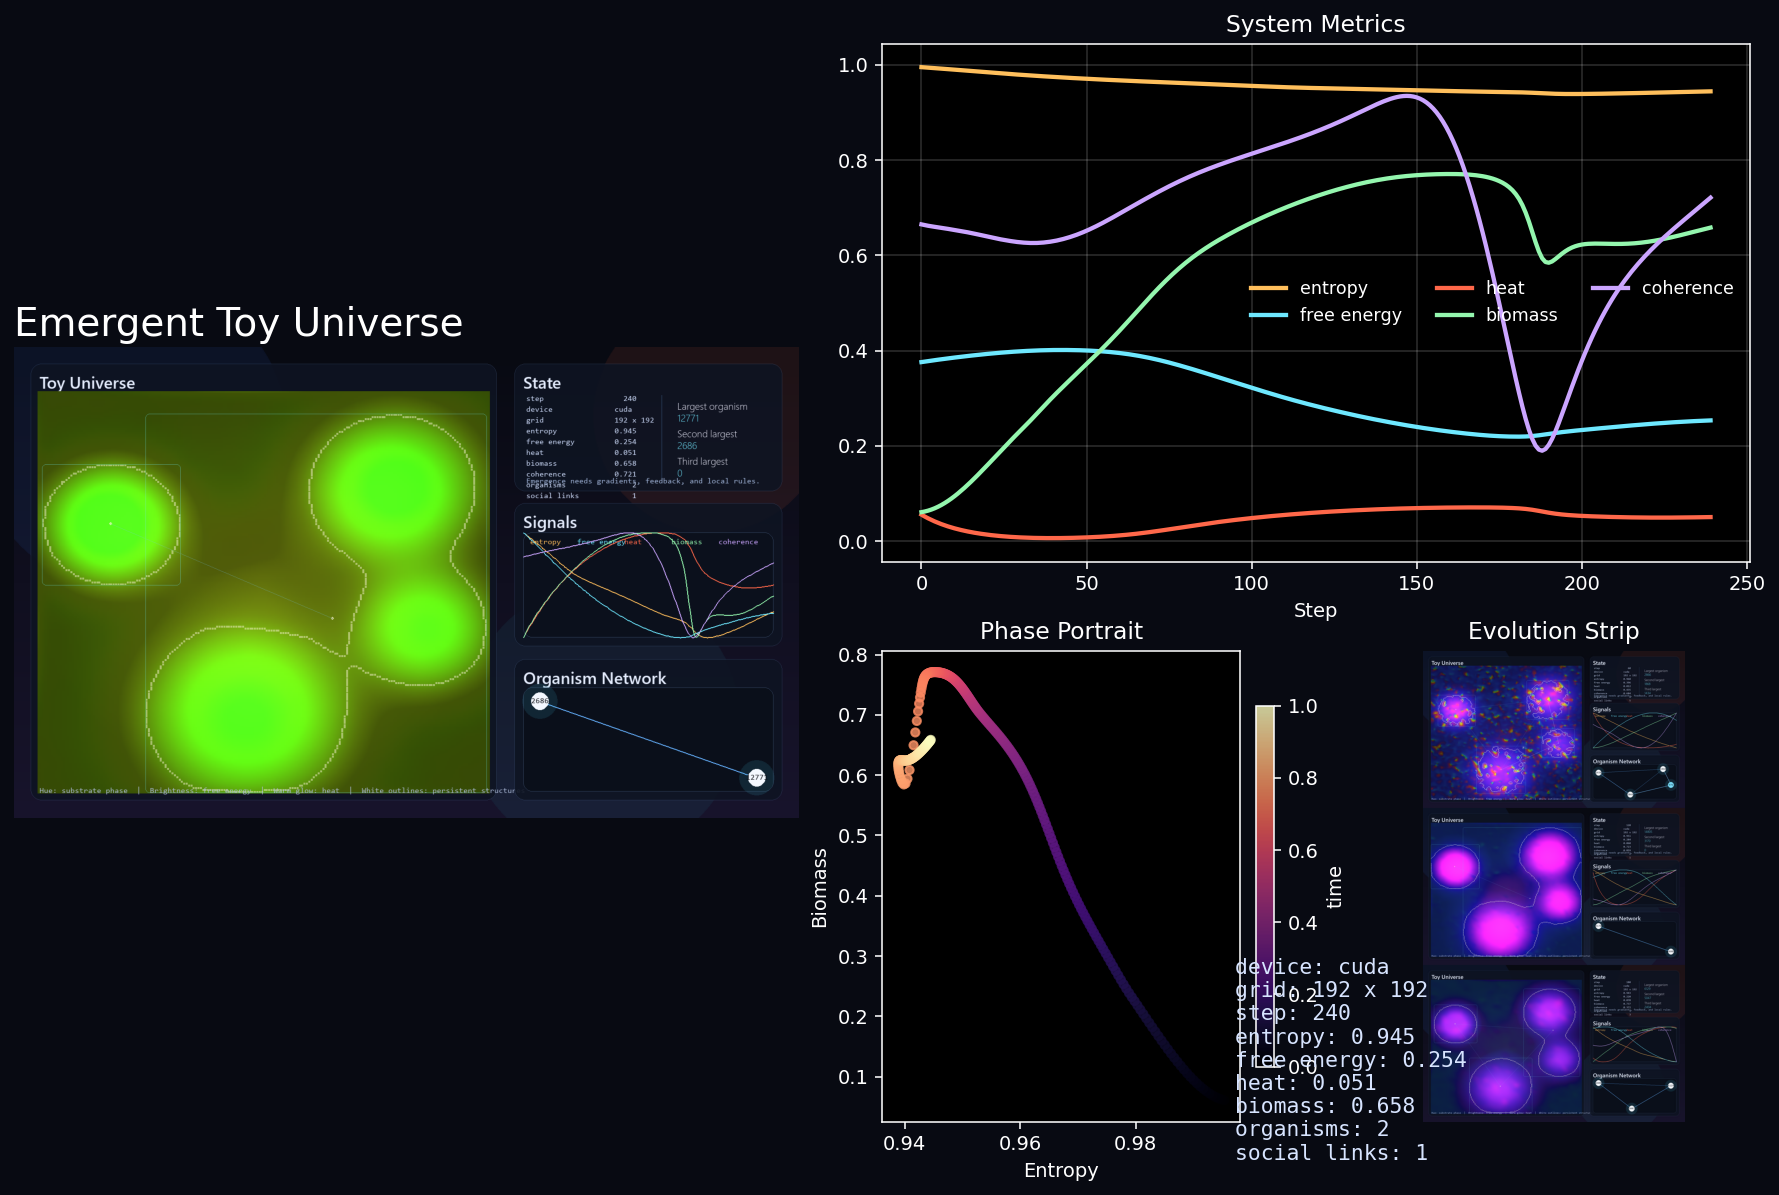
\includegraphics[width=0.95\textwidth]{artifacts/toy_universe_showcase.png}
\caption{Poster from the simpler \texttt{toy\_universe.py} simulation
(same physics and chemistry, no neural brains or science engine).
\textbf{Top-right}: System metrics over 250 steps.
\textbf{Bottom-left}: Phase portrait (entropy vs biomass).
\textbf{Bottom-right}: Evolution strip (three snapshots).}
\label{fig:showcase}
\end{figure}

\paragraph{World panel (large left image).}
We see four bright, roughly circular ``organisms'' glowing
vivid green-yellow against a dark background.
These are the connected components — life-mask blobs — detected
at step 250.
Their colours (hue from phase, brightness from free energy)
are relatively uniform \emph{within} each blob but differ
\emph{between} blobs, reflecting that each organism sits
in a slightly different phase domain of the psi field.
The glowing halos around each blob are the bloom effect
from high-brightness pixels.
The dark border is the vignette.

White outlines delineate the life-mask boundaries precisely.
Lines connecting organism centroids are the social-graph edges:
the blue-green colour indicates cooperative relationships
(high signal match, low heat).

\paragraph{System metrics (top right).}
The \textbf{entropy} (yellow/orange) curve
starts high (random initial state, broadly distributed energy),
then decreases as energy concentrates near the star sources,
then stabilises.
This is classic self-organisation: a disordered initial state
spontaneously develops spatial structure, reducing entropy.

The \textbf{free energy} (cyan) rises quickly as the source map
injects energy, then plateaus once metabolic consumption
by the growing biomass balances the source input.

The \textbf{heat} (red) grows slowly throughout — the system
warms up as metabolism converts free energy to waste heat.
That it remains below 0.3 throughout is the signature of
effective edge cooling.

The \textbf{biomass} (green) follows an S-shaped growth curve:
slow initial nucleation, rapid growth,
then saturation as the life potential is limited by heat and
available free energy.

The \textbf{coherence} (purple) starts from random initialisation
near $0.5$ (equal probability of all four psi channels having
moderate norm) and evolves as the orthogonal gates create
organised phase domains.

\paragraph{Phase portrait (entropy vs biomass).}
The scatter plot traces the simulation's trajectory
through (entropy, biomass) space.
Early frames (dark points) cluster at high entropy,
low biomass — random chaos before life takes hold.
Later frames (bright points) shift toward lower entropy,
higher biomass — the attractor of the system.
The arrow-like shape of the trajectory shows that
as biomass grows, entropy falls;
this is the information-theoretic signature of
\textbf{biological organisation reducing disorder locally}.
(Note: globally the entropy still increases — the heat dissipated
through the edges more than compensates. The second law is respected.)

\paragraph{Evolution strip.}
Three snapshots at steps 90, 180, and 270.
The organisms are clearly visible from the first snapshot
onwards, confirming that persistent structures form early
and are maintained throughout the run.
The increasing brightness over time reflects the growing
free-energy concentration.

\subsection{The Full Emergent Universe Engine (Figure~\ref{fig:full_dashboard})}

\begin{figure}[h]
\centering
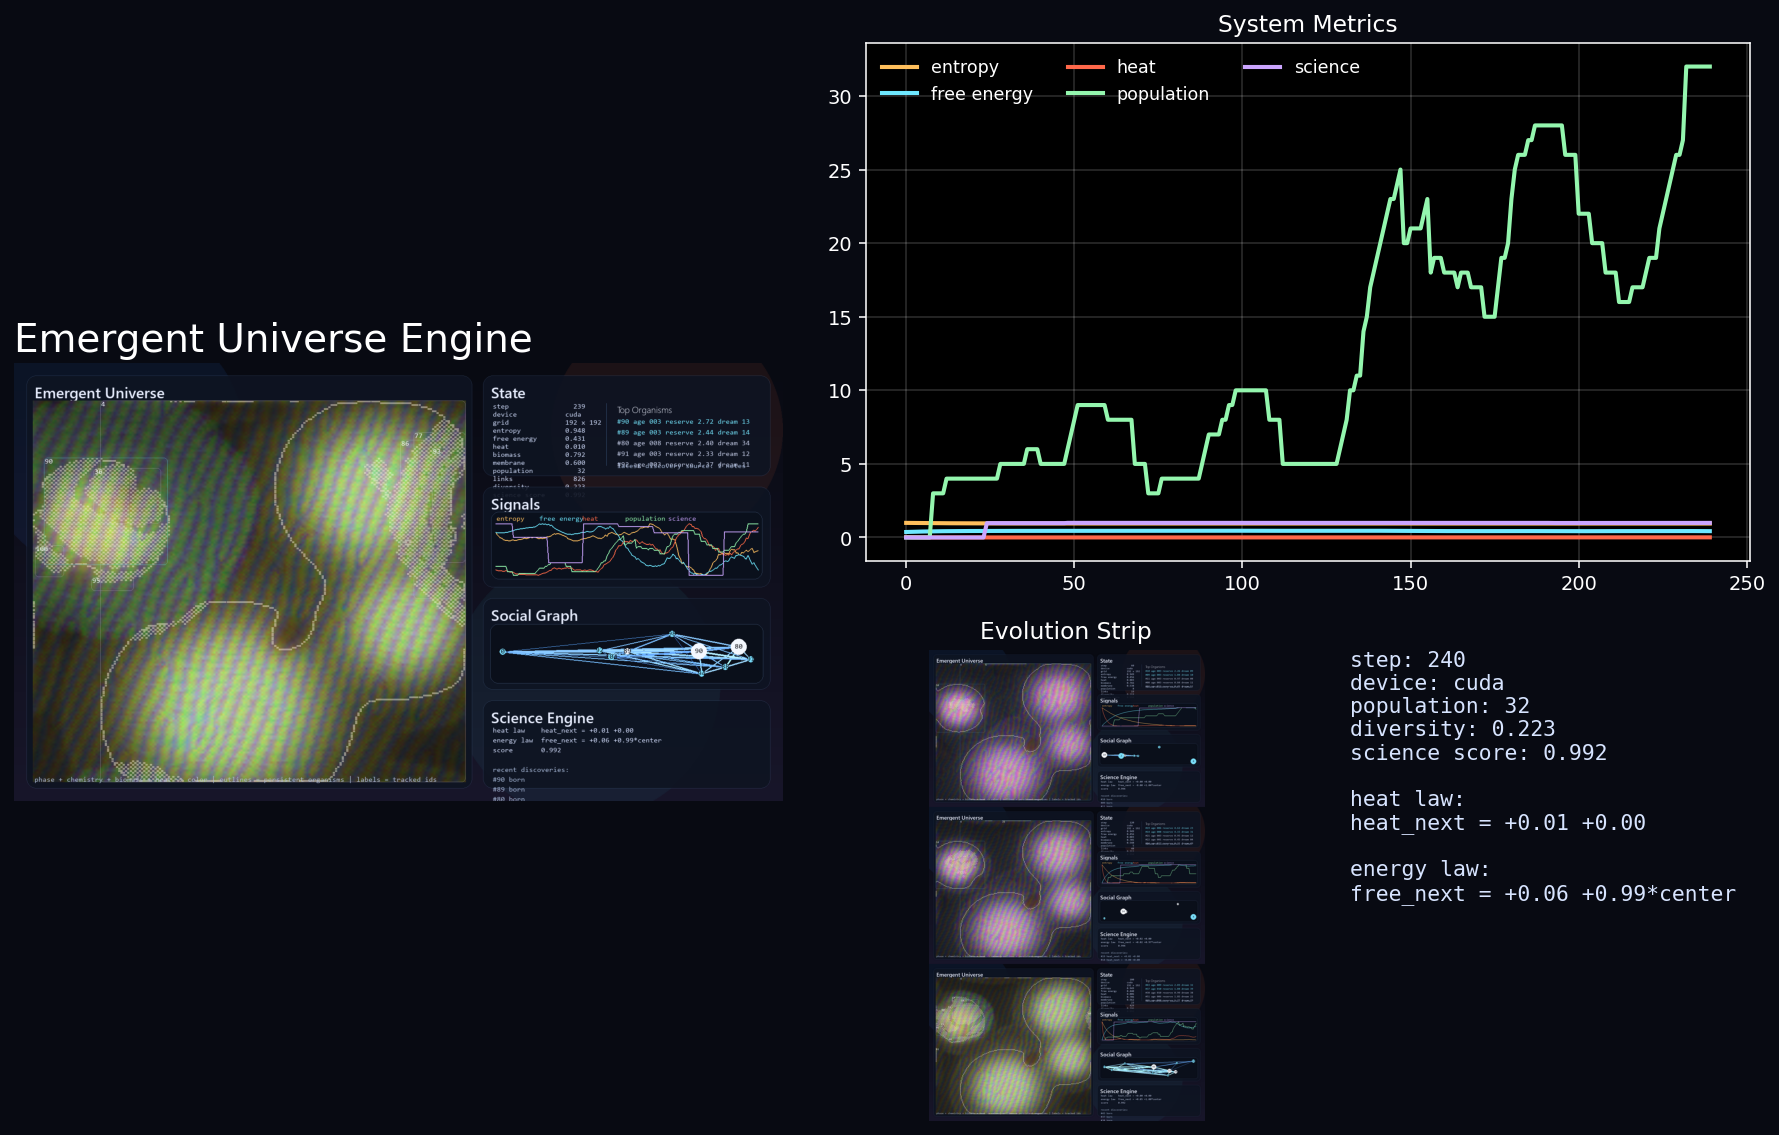
\includegraphics[width=0.95\textwidth]{artifacts_full/emergent_universe_full.png}
\caption{Poster from the full \texttt{main.py} simulation at step 240
(CUDA, seed 7, $192\times192$, science score 0.992).
The world panel shows the live dashboard with neural organisms,
social graph, and science engine.
\textbf{Top-right}: System metrics.
\textbf{Bottom-right}: Discovered laws.}
\label{fig:full_dashboard}
\end{figure}

\paragraph{World panel.}
The universe in the full simulation looks similar to the toy version
in large-scale structure (bright blobs on dark background,
phase-coloured domains),
but the dynamics are richer: organisms have moved (note the
slightly irregular blob shapes from neural-directed motion),
membranes are visible as sharper blob boundaries,
and the trail effect creates a slight smear showing
recent organism trajectories.

The ID labels (numbers in white) identify tracked organisms
by their \texttt{organism\_id}.
The fact that IDs are small (1-digit or 2-digit) and correspond
to a population of 12 alive organisms (as shown in State panel)
means most of the early random organisms have died and been
replaced by the fitter evolved descendants.

\paragraph{Population curve (green, system metrics).}
The most striking feature of the full simulation metrics
is the \textbf{population oscillation}: it shows large swings
(from near 0 to $\sim$32 and back).
These oscillations are a signature of \emph{boom-bust cycles}:
\begin{enumerate}[nosep]
\item Population grows, consuming free energy.
\item Free energy drops; heat rises.
\item Organisms start failing the life mask (heat too high, energy too low).
\item Mass die-off; environment recovers.
\item Free energy rises again; new organisms nucleate.
\item Repeat.
\end{enumerate}
This is a classic predator-prey type oscillation,
here between the organisms (consumers) and the energy field (resource),
analogous to the Lotka-Volterra equations of ecology.

\paragraph{Science score (purple).}
The science score climbs steeply and reaches 0.992 —
near-perfect law discovery.
This means the evolutionary regression algorithm has found
a linear combination of the 7 features that predicts
the next-step heat and free energy with very high accuracy.
Looking at the text panel:

\begin{quote}
\texttt{heat law: heat\_next = +0.01 +0.00}\\
\texttt{energy law: free\_next = +0.06 +0.99*center}
\end{quote}

The energy law $F_{t+1} \approx 0.06 + 0.99\,F_t$ captures
the dominant effect: free energy at a cell is strongly
autocorrelated (yesterday's value predicts tomorrow's,
with a small upward drift from the source).
This is a quantitatively correct first-order description of
the diffusion-and-source dynamics of equation~\eqref{eq:F}.
The science engine has ``discovered'' a conservation-like law
governing the universe's energy field.

\paragraph{Social Graph panel.}
The social graph shows a small network of 6--8 nodes with
several edges.
Node size is proportional to organism area (larger blobs = larger nodes).
Edge colour ranges from blue (low trust) to teal/cyan (high trust).
The presence of thick, bright edges means some organisms
have maintained sustained cooperative contact over many steps —
they have accumulated trust through repeated energy-sharing
and signal-compatible interactions.
These are the organisms most likely to have undergone sexual
reproduction with each other,
blending their genomes and sharing discoveries.

% ============================================================
\section{The Toy Universe vs the Full Engine: A Comparison}
% ============================================================

\begin{table}[h]
\centering
\renewcommand{\arraystretch}{1.3}
\begin{tabular}{lll}
\toprule
\textbf{Feature} & \textbf{toy\_universe.py} & \textbf{main.py (full)} \\
\midrule
Physics engine & Simple rotation matrix & Brick-wall orthogonal gates \\
Organism tracking & Shape + area only & Full OrganismRecord with genome \\
Neural brains & None & 2-layer MLP + world model + dreaming \\
Evolution & None & Mutation, sexual recombination \\
Social network & Proximity + signal edges & Full trust/conflict/cooperation \\
Science engine & None & Symbolic regression via ES \\
Diversity metric & None & Mean pairwise genome distance \\
\midrule
Code lines (approx.) & $\sim$900 (monolithic) & $\sim$1500 (modular) \\
Emergent phenomena & Phase patterns, GS life & All of the above + ecology \\
\bottomrule
\end{tabular}
\caption{Comparison between the two simulation versions.}
\end{table}

The toy universe is a clean, self-contained demonstration
of how phase patterns, reaction-diffusion chemistry, and
free-energy thermodynamics alone produce persistent
spatial structures without any higher-level machinery.
The full engine builds an entire biological stack on top.

% ============================================================
\section{Key Mathematical Concepts — Quick Reference}
% ============================================================

This section collects the essential mathematical ideas
used throughout, in one place.

\subsection{The Discrete Laplacian and Diffusion}

On a 2D grid, the Laplacian operator is discretised as:
\[
  (\nabla^2 f)_{i,j} = f_{i+1,j} + f_{i-1,j}
    + f_{i,j+1} + f_{i,j-1} - 4\,f_{i,j}.
\]
This is implemented as a $3\times3$ convolution with kernel
$\bigl[\begin{smallmatrix}0&1&0\\1&-4&1\\0&1&0\end{smallmatrix}\bigr]$.
Circular (periodic) boundary conditions wrap the grid edges.
Adding $\alpha\,\nabla^2 f$ to $f$ per step implements
\textbf{discrete diffusion} with diffusivity $\alpha$.
In the continuum limit, this is the heat equation
$\partial_t f = \alpha\,\nabla^2 f$.

\subsection{The Sigmoid and Its Relatives}

The \textbf{logistic sigmoid}:
\[
  \sigma(x) = \frac{1}{1+e^{-x}},\quad
  \sigma : \RR \to (0,1).
\]
Used for probabilities and smooth thresholds.

The \textbf{tanh}:
\[
  \tanh(x) = \frac{e^x - e^{-x}}{e^x + e^{-x}} = 2\sigma(2x) - 1,
  \quad \tanh : \RR \to (-1,1).
\]
Used for neural activations (bipolar, bounded).

The \textbf{ReLU}:
\[
  \relu(x) = \max(0, x),
\]
used for one-sided effects (``only if positive'').

\subsection{Shannon Entropy}

Given a probability distribution $p_i = f_i / \sum_j f_j$,
the Shannon entropy is:
\[
  H = -\sum_i p_i \log p_i.
\]
Normalised by $\log N$ (where $N$ is the number of cells)
to give $H \in [0,1]$.
$H\approx 1$ means energy is uniformly spread;
$H \approx 0$ means all energy is concentrated in one cell.
Biological self-organisation corresponds to
\emph{decreasing} entropy as energy concentrates in living structures.

\subsection{Orthogonal Matrices from QR Decomposition}

To generate a random orthogonal matrix $Q$:
\begin{enumerate}[nosep]
  \item Sample $A \sim \mathcal{N}(0, I_{n\times n})$.
  \item Compute QR decomposition: $A = QR$.
  \item If $\det(Q) < 0$, flip the sign of one column: $Q_{:,0} \leftarrow -Q_{:,0}$.
\end{enumerate}
This samples uniformly from the Haar measure on $O(n)$
(the uniform distribution on the orthogonal group) —
no direction is privileged.

\subsection{Gaussian Deposition}

Depositing a Gaussian ``blob'' at position $(x_0, y_0)$:
\[
  \text{field}(x,y) \;\mathrel{+}=\;
  A\,\exp\!\Bigl(-\frac{(x-x_0)^2+(y-y_0)^2}{2\sigma^2}\Bigr).
\]
This is the standard Gaussian kernel.
In the code, organism actions are deposited as Gaussian blobs
so that their effects spread smoothly over a few neighbouring cells.

\subsection{Connected-Component Labelling via BFS}

Breadth-first search on the binary mask:
for each unvisited live cell, expand to 4-connected neighbours
iteratively until no more live neighbours remain.
Time complexity: $O(N^2)$ per scan (each cell visited once).
In practice, for sparse masks on a $192\times192$ grid,
this is very fast.

% ============================================================
\section{Physical Analogies and Inspirations}
% ============================================================

The simulation draws on a rich tradition of physics and
complex systems:

\begin{description}
  \item[Quantum field theory] The $\bpsi$ field is inspired
    by the wave function, with orthogonal gates mimicking
    unitary time evolution.
    The phase $\varphi$ and coherence $\kappa$ mirror
    phase and amplitude in quantum mechanics.

  \item[Statistical mechanics] The thermodynamic engine
    captures the first and second laws: energy is conserved
    (flow is tracked), entropy increases globally
    (waste heat accumulates and escapes).
    The simulation is a non-equilibrium statistical system
    maintained by the source map.

  \item[Morphogenesis] The Gray-Scott chemical system is a
    direct descendent of Turing's 1952 reaction-diffusion model.
    The patterns it produces (spots, stripes, spirals)
    appear in animal coats, sea-shell markings, and
    embryonic tissue.

  \item[Ecology] The population oscillations, predator-prey
    dynamics, cooperation/competition trade-offs, and
    genetic diversity all have direct analogues in
    mathematical ecology (Lotka-Volterra, evolutionary game theory).

  \item[Cognitive science] The MLP neural brain, world model,
    and dreaming are simplified versions of Hebb's rule,
    model-based RL, and sleep consolidation in neuroscience.

  \item[Cultural evolution] The discovery propagation
    through the social network mirrors the spread of knowledge
    through human societies.

  \item[Philosophy of science] The science engine is a
    computational toy model of Karl Popper's falsificationism
    and Thomas Kuhn's paradigm shifts, operating inside a
    simulated universe.
\end{description}

% ============================================================
\section{End-to-End Walk-Through of One Simulation Step}
% ============================================================

Let us trace exactly what happens in one time step
of the full engine, starting from state $\mathbf{S}_t$:

\begin{enumerate}

\item \textbf{Physics.}
  The psi field $\bpsi$ is updated via the
  orthogonal gate (horizontal or vertical, alternating),
  then diffusion, mixing, curl, drive, and damping
  (equation~\eqref{eq:psi}).
  Phase $\varphi$, coherence $\kappa$, and matter type $m$
  are recomputed.

\item \textbf{Thermodynamics.}
  Snapshots of $F_t$ and $T_t$ are saved.
  New $F_{t+1}$ and $T_{t+1}$ are computed
  (equations~\eqref{eq:F}--\eqref{eq:T})
  using energy demand $D_t$ set by organisms in the previous step.

\item \textbf{Cellular Life.}
  Chemical species $a, b, n$ are evolved by the extended
  Gray-Scott equations.
  Biomass $\beta$ and membrane $\mu$ are updated.
  Signal $s$ is updated; energy demand $D$ is augmented by
  $0.02\,ab^2 + 0.03\,\relu(\beta-0.30)$.

\item \textbf{Organism Manager} (every 4 steps).
  The life mask is computed.
  BFS finds connected components.
  Existing organisms are matched or aged.
  Unmatched clusters spawn new organisms.
  Stale/starved organisms die.
  Diversity is recomputed.

\item \textbf{Drive reset.}
  Energy demand, signal drive, and repair drive are zeroed
  so organisms start fresh this step.

\item \textbf{Neural Brain.}
  Each alive organism:
  \begin{enumerate}[nosep]
    \item Observes its local field values.
    \item If memory is non-empty: compute reward, store experience,
      update world model (equation~\eqref{eq:worldmodel}).
    \item Compute action via MLP (equation~\eqref{eq:mlp}).
    \item Apply action: move, deposit signal/repair/energy demand.
    \item Update energy reserve.
    \item If cool and energy-rich: dream (MPC planning).
  \end{enumerate}

\item \textbf{Evolution.}
  Each age-eligible organism with sufficient energy reproduces.
  Partner selection, genome blending, or mutation.
  Child organism placed and seeded.
  Senescent starved organisms killed.

\item \textbf{Social Network.}
  All edges decay.
  Nearby pairs interact: cooperation, competition, energy transfer.
  Knowledge is transferred along high-trust edges.

\item \textbf{Science Engine.}
  48 new field samples are appended to the dataset.
  Every 24 steps, evolutionary regression finds the best
  linear law for heat and energy.
  Law is stored; lead scientist's discoveries updated.

\item \textbf{Metrics.}
  Entropy, free energy, heat, biomass, coherence, membrane,
  population, links, diversity, and science score are
  appended to history.

\item \textbf{Rendering.}
  The HSV composite image is computed from phase, chemistry,
  and energy fields.
  The trail is updated.
  The dashboard frame is rendered.
  The frame is stored for GIF output.

\end{enumerate}

% ============================================================
\section{Conclusion: What Has the Simulation Achieved?}
% ============================================================

The Emergent Universe Engine is a tour de force of
layered complexity.
Starting from nothing but a random Gaussian field and a fixed
star map, it spontaneously develops:

\begin{itemize}
  \item \textbf{Physical structure:} phase domains, vortices,
    and domain walls in the psi field,
    driven by the orthogonal gate dynamics.

  \item \textbf{Chemical patterns:} Turing-like spots and stripes
    in the activator field $b$, mediated by the
    asymmetric diffusion of the Gray-Scott system.

  \item \textbf{Energetic gradients:} steady-state spatial
    distributions of free energy and heat, maintained far from
    equilibrium by the four star sources and edge cooling.

  \item \textbf{Living structures:} persistent, self-maintaining
    regions of high biomass and membrane formation,
    identified as organisms via connected-component labelling.

  \item \textbf{Behaviour:} organisms move, harvest, signal,
    and repair, guided by neural networks whose weights
    are part of their heritable genome.

  \item \textbf{Learning:} world models are updated online from
    experience; dreaming refines action biases toward
    reward-maximising policies — all without any
    pre-programmed objective.

  \item \textbf{Darwinian evolution:} the population's genome
    distribution drifts under selection pressure imposed by
    the thermodynamic environment, with both asexual mutation
    and sexual recombination as generators of variation.

  \item \textbf{Social complexity:} organisms form trust
    relationships, cooperate, compete, and share knowledge,
    producing an emergent social network.

  \item \textbf{Science:} the simulation's own organisms
    effectively rediscover approximate quantitative laws
    describing how its fields evolve —
    an in-universe empirical science program.
\end{itemize}

None of these phenomena are explicitly programmed.
Each is an \emph{emergent consequence} of the layer below it.
Phase patterns enable chemical patterns; chemical patterns
enable life; life enables evolution; evolution enables
intelligence; intelligence enables social networks;
social networks enable cultural knowledge diffusion.

\begin{tcolorbox}[keybox={The central lesson}]
\textbf{Emergence is not a mystery — it is a consequence.}
Given the right substrate (energy gradients, nonlinear interactions,
diffusion, feedback), complexity does not have to be designed:
it \emph{has} to appear.
The question for the designer of a complex system is not
``how do I make this happen?'' but
``how do I not accidentally prevent it from happening?''
The Emergent Universe Engine answers that question by
getting out of the way: it provides minimal ingredients
and lets the physics do the rest.
\end{tcolorbox}

The simulation's code is a remarkably concise implementation
of this philosophy.
Each engine module is $\sim$50--150 lines of PyTorch.
The physics fits in one function.
The thermodynamics in ten lines.
The cellular life in $\sim$25 equations.
Yet together they produce a system whose long-term behaviour
nobody fully predicted when writing the equations —
which is, of course, exactly the point.

\bigskip
\hrule
\bigskip
{\small
\noindent\textbf{Simulation parameters used in the figures:}
grid size $192\times192$; 360 simulation steps; random seed 7;
device: CUDA (NVIDIA GPU); internal dimension $d=4$;
chemical dimension 3; hidden layer size 12; action size 6;
observation size 11; max organisms 32; max memory 32;
sample every 4 steps; organism refresh every 4 steps;
science period 24 steps; FPS 30.
}

\end{document}
